\section{Lack of features in the model}

\label{sec:lack}
When we started to implement the model and simulate our two cases, we encountered some
problems that we did not foresee when we read the article \cite{self-org}, and the other
articles \cite{helbing00}, \cite{social-force}.
We encountered some special cases where the model did not suffice to give a realistic
simulation, and also we could not, from the articles, figure out how to fix some initial parameters.
In the articles the authors did not write of any such problems and how to deal with them,
so we had to come up with our own solutions to solve them, and thereby give a more realistic
simulation.
In the following section we discuss these problems and our solutions to these problems.

\subsection{Discussion on walls in special cases.}\label{wallEndpoints}
The wall is created as a vector. The repulsive force vector is perpendicular to the wall 
vector and has a direction directly towards the pedestrian $\alpha$.

In the general case of the repulsive force on an agent, $\alpha$, from a wall 
nearby is given as a function of the vector from the nearest point. This point we 
calculate by finding the point that makes the vector form $\alpha$ to the wall be 
perpendicular to to vector that is the wall. In some cases though the point will not 
be on the wall it self. This of course makes no sense since the agent would then be 
repulsed by a non existing part of the wall meaning that it would avoid free 
areas. In this case we would have to use the end point of the wall. But doing this 
can make some unrealistic behaviour as well, if the walls have the right composition. 

Let's start out by looking at a case with no problem. A case with no problems is a 
room where the angles between the walls is less than $180^o$, i.e. a squared room 
where the angles are $90^o$. For a pedestrian close to the corner between two walls, we 
would calculate the repulsive force from both of the walls. By doing this, we can avoid 
the agents to go through either one of the walls. Then we get a force directly away 
from each of the walls. This clearly makes sense and there is no problem in doing so.

\subsubsection{Forces at kinks}
The case where the angle between two walls is greater than $180^o$ could on the 
other hand give some problems if not handled correctly. The case is sketched in 
figure \ref{fig:wallcase}. Here there are 3 different areas that a pedestrian $\alpha$ 
can be in. The area A where $\alpha$ is only perpendicular to wall $1$, in area B, 
$\alpha$ will not be perpendicular to any of the walls and in C he will be only 
perpendicular to wall 2. 

If a pedestrian is in area B then we would calculate the 
forces from the end point of the walls. This will be from the point where the two 
walls meet. This will give a double repulsion from one point and that 
does not make sense. Also when the agent is in are A or C it would get a repulsive force 
from a second wall it would be of no risk of going into and in many situations 
could not see because the first wall is blocking the sight. This of course does not 
make any sense either. So the way that we handle this situation is the following. 
When the angle between the walls is greater than $180^o$, from agent $\alpha$'s 
point of view, it should look at the two walls as one, and in that way it will 
only calculate one force from the walls. In area A or C only the closest point 
on the closest wall should affect it. In the case of $\alpha$ being in area B 
the walls themselves does not matter, only the vector going from the conjoint 
point of the walls to $\alpha$, should affect and only one time. Doing this, 
there should be no unrealistic scenarios concerning wall junctions and walls 
with more than $180^o$ between them. But this could create undesired 
behaviour at doors of other objects created with free end points.

\begin{figure}[ht]
\centering
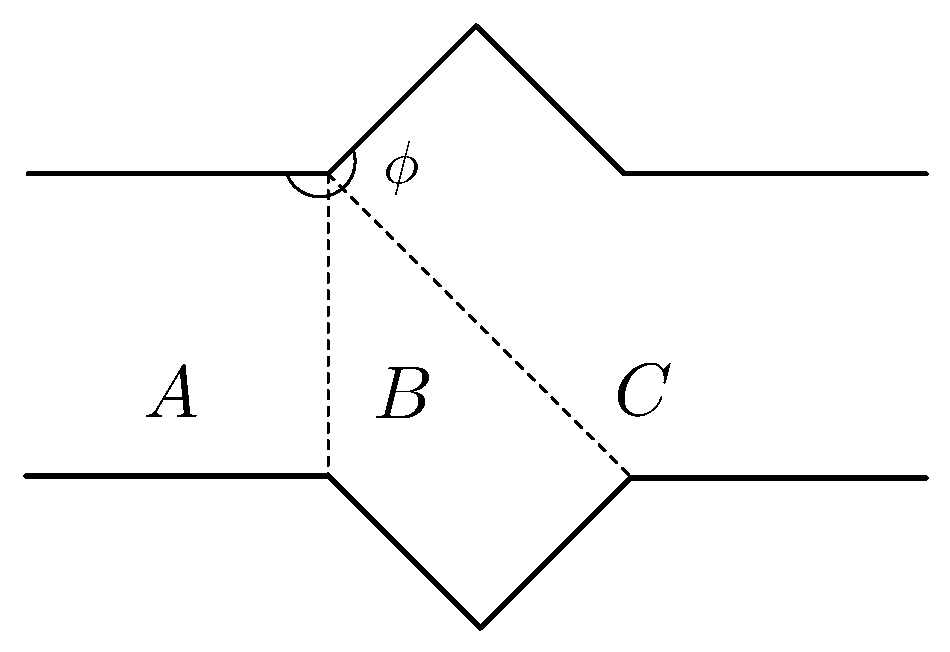
\includegraphics[scale=0.45]{Figures/WallCase.pdf} 
\caption{}\label{fig:wallcase}
\end{figure}

\subsubsection{The force at doorways}
We encountered a problem when dealing with doors. The problem arises because 
the door is constructed by two free endpoints and an agent feels two repulsion 
forces from these points according to section \ref{wallEndpoints}. This means 
that a pedestrian trying to exit through the door will feel repulsive forces 
from both of the walls which prevent it from walking through the door. The moment it 
passes through the door it will be pushed forward and accelerate which is unwanted 
behaviour. This we resolved by removing the force from free endpoint when:

\begin{equation}
\| p - w \| > R
\end{equation}
where $ p $ is the position of the agent, $ w $ is the position of the door's endpoint, 
and $ R $ is the radius of the agent.

This creates what we could call a "non repulsion zone" see figure(Mikkel Lav Tegning!).
In rare cases it could happen that an agent is trying to exit the room and it feels 
no repulsion because it is in the "non repulsive zone", and it is then pushed sideways out 
of the "non repulsion zone" and suddenly it will feel a great repulsive force because 
it first "discovers" the force when it is very close to the wall see figure(Mikkel Lav Tegning!).

\subsubsection{Calculating the repulsion from walls}
\label{sec:repulsion-points}
The calculation of repulsion from the walls is split in two parts for each 
agent: First all the points on the walls that will affect the agent is 
identified, then the repulsion from each point is calculated. As explained in 
section~\ref{sec:the-model}, the repulsion from the wall is measured from the 
nearest point of the wall to the actor. Identifying these points is done using 
the following algorithm:

\begin{enumerate}
    \item For each wall, calculate the projection of the vector pointing from 
        the wall's starting point to the agent, unto the vector pointing from 
        the wall's starting point to its endpoint.
        \begin{enumerate}
            \item If this point is part of the wall, save it to the list of points 
                repulsion should be calculated from, and add the wall's two endpoints 
                to the list of already used endpoints.

            \item If the projected point is not part of the wall, the endpoint closest 
                to the agent is used instead. This endpoint is saved to a 
                third list of endpoints repulsion should be calculated from.
        \end{enumerate}

    \item After having gone through all walls, for each point in the third 
        list, check if this point is already in the list of used endpoints. If 
        so, discard it. Otherwise, add it to the list of points repulsion 
        should be calculated from, and to the list of used endpoints.
\end{enumerate}

The algorithm starts out with the list of walls, and produces a list of points 
to calculate this repulsion from, ensuring that no wall endpoint is used 
twice. The points are then used as a basis for calculating the repulsion, as 
described in section~\ref{sec:the-model}.

\subsection{Initial conditions and constants}
\label{sec:init-cond}
% TODO: Go through all the constants and add where we got it from; either a 
% reference or saying that we came up with it ourselves.
When initialising the model, parameters are set for each agent. In the 
model, every parameter can vary between actors, while in practice many of them 
do not. In this section, we go through the parameters and how they are set.  
For all random numbers, the operating system's built-in random number 
generator is used and considered to be sufficient for our purposes. We run 
multiple simulations of the same initial conditions by fixing the seed of the 
random number generator to the same value for each run. Distributions are 
drawn by using the distribution functions of the \emph{NumPy} mathematical 
library for Python \cite{numpy}.

\subsubsection{Position related parameters}
There are a number of parameters that are set that have to do with the initial 
position of actors and walls. Some are given, and some we had to come up
with ourselves. They are:

\begin{itemize}
    \item \textbf{Wall endpoints:} Points describing the endpoints of the 
        walls. They are set according to the scenario we want to simulate, so 
        in a square room with a single exit in the middle of a wall, there 
        will be five wall segments.

    \item \textbf{Agent positions:} Each agent has a starting position 
        distributed randomly within the room. They are created by drawing a 
        set of random numbers for the x and y coordinates respectively, and 
        adjusting the range of this random number to be within the room's 
        dimensions. Agents' positions are adjusted so that they do not overlap 
        with the walls by adjusting coordinates so that the distance from the 
        center of each agent to each wall is at most the radius. This 
        adjustment is not made between agents, so they may overlap initially. 
        It is assumed that the model will correct this within the first few 
        simulation steps, which is also what we have seen in practice.

    \item \textbf{Agent's radius:} The agent's radius is drawn from a normal 
        distribution with a mean of $0,3$ meters and a standard deviation of 
        $0,05$ meters. This is done to simulate a natural variety in the width 
        of human shoulders, and to avoid deadlocks caused by perfectly 
        symmetrical forces that might otherwise occur \cite{helbing00}.
        %TODO: Check this reference, maybe better explanation?
\end{itemize}

\subsubsection{Movement related parameters}
A number of parameters are set to control the movement of the agents. They 
are:

\begin{itemize}
% TODO: Add a section about placement of waypoints.
%   Square room: Place the waypoint at or just outside the exit.
%   Corridor: Place the waypoint a long distance away, so that pedestrians 
%   move almost in a straight line along the corridor.
    \item \textbf{Waypoint:} We think of this setup that suits each scenario  
        by ourselves. Each agent has a waypoint that they move towards, 
        and is the same for all agents when there is only one exit. 
        For a square room, this waypoint is set just outside the exit the agent 
        will move towards. For a corridor, the waypoint is put at a position 
        far away from the corridor and along the line that the corridor lies, so that
        there is no traffic rules for each agent such as to stick to the right or left.
        
        %where there are multiple exits, actors are set to move towards one of 
        %the exits at random, regardless of their position within the room. 
        Since the model does not deal with pathfinding, waypoints are not 
        changed during the simulation. When an agent reaches its waypoint, it is 
        considered to have escaped, and is removed from the simulation.

    \item \textbf{Initial velocity:} The initial velocity does not matter much 
        because the agent can quickly adjust its velocity during the first few 
        step sizes, and there is no recommends from the articles. 
        Our way of getting the initial velocity is by setting both a vector and a scalar 
        representing vector length. The scalar velocities are drawn from a 
        normal distribution with a mean of $1.34$ and a standard deviation of 
        $0,26$. The initial velocity vectors are created by multiplying the 
        scalar velocity with a normalised vector pointing from the agent's 
        initial position to the waypoint.
        % TODO: Where do the mean and deviation come from?

    \item \textbf{Desired speed $  V_{i}^{0}  $:} The desired speed is 
        the speed the agent wants to move at (see the explanation in 
        section~\ref{sec:the-model}). The desired speed at $ t=0 $ is set 
        equal to the initial speed 
        under our assumption that when people start to leave a room they will 
        initially (try to) move with their desired speed, and then be 
        affected by the model parameters once they start moving.

    \item \textbf{Maximum desired speed $ V_{i}^{max} $:} The maximum 
        desired speed depends on its desired speed as $ V_{i}^{max} =1.3 V_{i}^{0}  $.
       c
        
    \item \textbf{Relaxation time $ \tau $:} The relaxation time is the time it would 
        take an unhindered agent to adjust to its desired velocity after 
        having been hindered by something blocking their path. This is set to 
        one second for all actors, in \cite{self-org}. However, in another article 
        \cite{helbing00}, the relaxation time is $ 0,5 $.

    \item \textbf{$\lambda$:} \cite{ABconstant} chose $\lambda$ $\approx 0.1$ 
        to take into account
    anisotropic character of pedestrian interaction, such that the situations 
    in front of
    a pedestrian have bigger impact on the pedestrians behaviour than things 
    going on
    behind them. 
    % TODO: Is this explanation correct?
\end{itemize}

\subsubsection{Constants} \label{constants}
The model includes a number of constants. These are parameters that do not 
vary between the agents, but are fixed for the whole simulation. They are:

\begin{itemize}
    \item \textbf{Timestep:} The timestep is the $\Delta t$ that passes for 
        each step of the simulation. As discussed in 
        section~ %TODO: Make new reference
		, there are various trade-offs in making 
        this parameter larger or smaller. We have experimented with different 
        values, and have found that a value of $0,01$ seconds makes for a 
        simulation without errors such as jitter that results from larger 
        timestep values. Since setting the timestep corresponds to setting a 
        delta value for an Euler integration, there are various methods that 
        originate from this integration method, that might be used to vary the 
        timestep dynamically during the simulation. 
         However, we have found 
        that with a fixed value of $0,01$ seconds, we get reasonable 
        performance of our simulation, so we have not found the need to 
        complicate our program by applying such methods.
        % TODO: Reference for dynamic timestep adjustment

    \item \textbf{$A$, $B$:} These values are given in \cite{ABconstant}. 
        Although the model allows for them to vary between agents, we have 
        (just as is done in the article) set them to a fixed value for the 
        whole simulation. The values given are $A_2=3,0$ and $B_2 = 0,2$.

    \item \textbf{$ U^{0} $:} While calculating the wall repulsive force, a potential
        constant $ U^{0} $ is needed to get the force. Though it will be realistic to 
        have a hard core potential \cite{self-org}, we have tried different values 
        of $ U^{0} $ so that the agents do not keep a too far distance from the wall 
        and they do not pass through the wall under normal conditions. In the end, 
        we choose $ U^{0} =2 $ .
 
\end{itemize}

